\documentclass[12pt,border=6pt]{standalone}
\usepackage{fontspec}
\setmainfont{BeVietnamPro}[Path=D:/IOT_Tools/downloads/fonts/,Extension=.ttf,UprightFont=*-Regular,BoldFont=*-Bold]
\usepackage{amsmath}
\usepackage{unicode-math}\setmathfont{Cambria Math}
\usepackage{xcolor}
\usepackage{tikz}
\usetikzlibrary{positioning,arrows.meta,shapes.geometric,shapes.misc,calc,fit,backgrounds,decorations.pathreplacing,shadows,3d,perspective}
\usepackage{tikz-3dplot}
\usepackage{pgfplots}\pgfplotsset{compat=1.18}
\usepgfplotslibrary{groupplots,fillbetween}
\definecolor{cDo}{HTML}{BB2025}\definecolor{cDoD}{HTML}{8E1418}\definecolor{cDoT}{HTML}{FCEBEC}
\definecolor{cXanh}{HTML}{326CE5}\definecolor{cXanhT}{HTML}{EAF0FC}
\definecolor{cLuc}{HTML}{15803D}\definecolor{cLucT}{HTML}{E6F4EA}
\definecolor{cVang}{HTML}{B45309}\definecolor{cVangT}{HTML}{FDF2E1}
\definecolor{cNavy}{HTML}{1E293B}\definecolor{cMuc}{HTML}{1F2937}\definecolor{cXam}{HTML}{4B5563}
\definecolor{cXamT}{HTML}{F3F4F6}\definecolor{cVien}{HTML}{DDE1E6}\definecolor{cTim}{HTML}{6D28D9}\definecolor{cTimT}{HTML}{F1EBFD}
\pgfplotsset{slide/.style={tick label style={font=\small}, label style={font=\small}, scaled ticks=false,
  /pgf/number format/fixed, /pgf/number format/use comma, /pgf/number format/1000 sep={\,},
  legend style={font=\small,draw=none,fill=none}, axis line style={cXam}, major tick style={cXam},
  grid style={cVien}}}
\pgfkeys{/pgf/number format/assume math mode=true}
\begin{document}
% F04 · S05 · trục thời gian 17/08 đến 26/11, 10 mốc (facts/06-tien-trinh.md mục (a)).
% Khung slide 17,9 x 5,6 in; vẽ theo inch thật, viền standalone 6 pt đã trừ.
% Ngày quy ra số ngày kể từ 17/08: 01/09=15, 01/10=45, 01/11=76, 26/11=101. X(d) = 0,35 + 0,1686 d.
\newfontface\semib{BeVietnamPro-SemiBold}[Path=D:/IOT_Tools/downloads/fonts/,Extension=.ttf]%
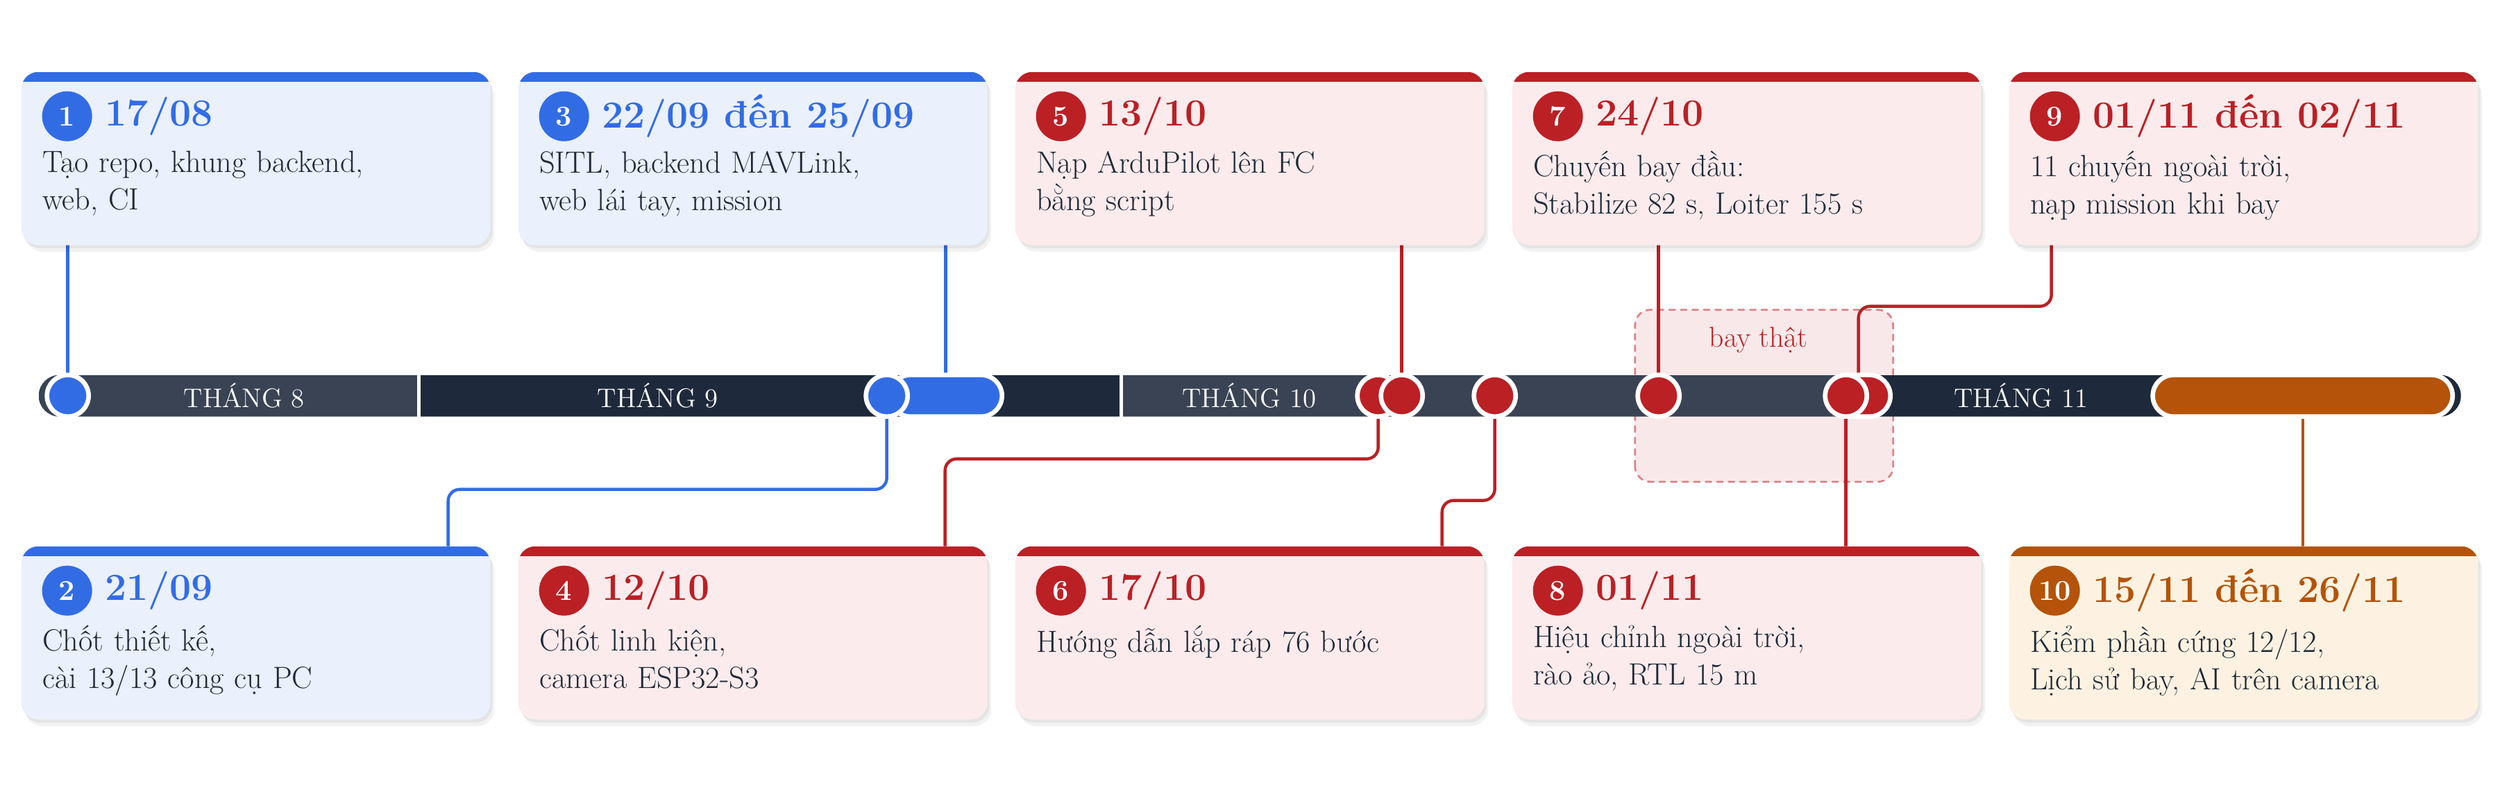
\begin{tikzpicture}[x=1in,y=1in,line cap=round,line join=round,
  sh/.style={general shadow={fill=black,opacity=.06,shadow xshift=1pt,shadow yshift=-1.6pt},
             general shadow={fill=black,opacity=.05,shadow xshift=2pt,shadow yshift=-3.4pt}}]
\frenchspacing
\useasboundingbox (0,0) rectangle (17.73,5.43);
\def\ay{2.715}
% ---------- thẻ mốc: \card{x trái}{y đáy}{số}{ngày}{mô tả}{màu}{nền}
\newcommand\card[7]{%
  \fill[#7,sh,rounded corners=9pt] (#1,#2) rectangle ++(3.38,1.25);
  \begin{scope}\clip[rounded corners=9pt] (#1,#2) rectangle ++(3.38,1.25);
    \fill[#6] (#1,#2+1.18) rectangle ++(3.38,0.07);\end{scope}
  \node[circle,fill=#6,text=white,inner sep=0pt,minimum size=0.36in,font=\fontsize{15}{15}\bfseries]
    at (#1+0.33,#2+0.93) {#3};
  \node[anchor=west,text=#6,font=\fontsize{20}{24}\bfseries,inner sep=0pt] at (#1+0.6,#2+0.93) {#4};
  \node[anchor=north west,text width=3.1in,align=left,text=cMuc,font=\fontsize{16}{19.5}\selectfont,inner sep=0pt]
    at (#1+0.15,#2+0.68) {#5};}
% ---------- dải "bay thật" 24/10 (d68) đến 02/11 (d77)
\fill[cDo,opacity=.10,rounded corners=8pt] (11.64,\ay-0.62) rectangle (13.50,\ay+0.62);
\draw[cDo!55,dashed,line width=1pt,rounded corners=8pt] (11.64,\ay-0.62) rectangle (13.50,\ay+0.62);
\node[text=cDo,font=\semib\fontsize{15}{15}\selectfont] at (12.53,\ay+0.40) {bay thật};
% ---------- đường nối thẻ ↔ mốc (vẽ trước để chấm đè lên)
\begin{scope}[line width=1.6pt,rounded corners=6pt]
  % trên: 1 3 5 7 9
  \draw[cXanh] (0.35,\ay) -- (0.35,3.80);
  \draw[cXanh] (6.675,\ay) -- (6.675,3.80);
  \draw[cDo]   (9.96,\ay) -- (9.96,3.80);
  \draw[cDo]   (11.81,\ay) -- (11.81,3.80);
  \draw[cDo]   (13.25,\ay) -- (13.25,3.36) -- (14.64,3.36) -- (14.64,3.80);
  % dưới: 2 4 6 8 10
  \draw[cXanh] (6.25,\ay) -- (6.25,2.04) -- (3.09,2.04) -- (3.09,1.63);
  \draw[cDo]   (9.79,\ay) -- (9.79,2.26) -- (6.67,2.26) -- (6.67,1.63);
  \draw[cDo]   (10.63,\ay) -- (10.63,1.96) -- (10.25,1.96) -- (10.25,1.63);
  \draw[cDo]   (13.16,\ay) -- (13.16,1.63);
  \draw[cVang] (16.45,\ay) -- (16.45,1.63);
\end{scope}
% ---------- trục tháng
\begin{scope}
  \clip[rounded corners=0.15in] (0.14,\ay-0.15) rectangle (17.59,\ay+0.15);
  \fill[cNavy!88!white] (0.14,\ay-0.15) rectangle (2.88,\ay+0.15);
  \fill[cNavy] (2.88,\ay-0.15) rectangle (7.94,\ay+0.15);
  \fill[cNavy!88!white] (7.94,\ay-0.15) rectangle (13.16,\ay+0.15);
  \fill[cNavy] (13.16,\ay-0.15) rectangle (17.59,\ay+0.15);
\end{scope}
\foreach \t in {2.88,7.94,13.16} \draw[white,line width=1.6pt] (\t,\ay-0.15) -- (\t,\ay+0.15);
\begin{scope}[text=white,font=\semib\fontsize{14}{14}\selectfont]
  \node at (1.62,\ay) {THÁNG 8};
  \node at (4.60,\ay) {THÁNG 9};
  \node at (8.86,\ay) {THÁNG 10};
  \node at (14.42,\ay) {THÁNG 11};
\end{scope}
% ---------- chấm / khoảng
\begin{scope}[line width=2.4pt]
  \filldraw[fill=cXanh,draw=white] (0.35,\ay) circle (0.15);
  \filldraw[fill=cXanh,draw=white,rounded corners=0.15in] (6.27,\ay-0.15) rectangle (7.08,\ay+0.15);
  \filldraw[fill=cXanh,draw=white] (6.25,\ay) circle (0.15);
  \filldraw[fill=cDo,draw=white] (9.79,\ay) circle (0.15);
  \filldraw[fill=cDo,draw=white] (9.96,\ay) circle (0.15);
  \filldraw[fill=cDo,draw=white] (10.63,\ay) circle (0.15);
  \filldraw[fill=cDo,draw=white] (11.81,\ay) circle (0.15);
  \filldraw[fill=cDo,draw=white,rounded corners=0.15in] (13.04,\ay-0.15) rectangle (13.48,\ay+0.15);
  \filldraw[fill=cDo,draw=white] (13.16,\ay) circle (0.15);
  \filldraw[fill=cVang,draw=white,rounded corners=0.15in] (15.37,\ay-0.15) rectangle (17.53,\ay+0.15);
\end{scope}
% ---------- 10 thẻ (trên: 1 3 5 7 9, dưới: 2 4 6 8 10)
\card{0.015}{3.80}{1}{17/08}{Tạo repo, khung backend,\\ web, CI}{cXanh}{cXanhT}
\card{3.595}{3.80}{3}{22/09 đến 25/09}{SITL, backend MAVLink,\\ web lái tay, mission}{cXanh}{cXanhT}
\card{7.175}{3.80}{5}{13/10}{Nạp ArduPilot lên FC\\ bằng script}{cDo}{cDoT}
\card{10.755}{3.80}{7}{24/10}{Chuyến bay đầu:\\ Stabilize 82 s, Loiter 155 s}{cDo}{cDoT}
\card{14.335}{3.80}{9}{01/11 đến 02/11}{11 chuyến ngoài trời,\\ nạp mission khi bay}{cDo}{cDoT}
\card{0.015}{0.38}{2}{21/09}{Chốt thiết kế,\\ cài 13/13 công cụ PC}{cXanh}{cXanhT}
\card{3.595}{0.38}{4}{12/10}{Chốt linh kiện,\\ camera ESP32-S3}{cDo}{cDoT}
\card{7.175}{0.38}{6}{17/10}{Hướng dẫn lắp ráp 76 bước}{cDo}{cDoT}
\card{10.755}{0.38}{8}{01/11}{Hiệu chỉnh ngoài trời,\\ rào ảo, RTL 15 m}{cDo}{cDoT}
\card{14.335}{0.38}{10}{15/11 đến 26/11}{Kiểm phần cứng 12/12,\\ Lịch sử bay, AI trên camera}{cVang}{cVangT}
\end{tikzpicture}

\end{document}
